\documentclass[pageno]{jpaper}

\newcommand{\IWreport}{Fall 2019}
\newcommand{\quotes}[1]{``#1''}


\widowpenalty=9999

\usepackage[normalem]{ulem}
\begin{document}

\title{Predicting NBA Records From Previous Season Stats}

\author{Sean Gai\\Adviser: Ben Raphael}

\date{}
\maketitle

\thispagestyle{empty}
\doublespacing
\begin{abstract}
This paper details a data analytics project that uses supervised machine learning to predict a given NBA team's regular season record using the team's previous season statistics. The project implements several regression techniques to build a variety of models and evaluates the performance of each one. This project aims to help general managers construct better rosters, coaches adopt new strategies, and sports bettors make more lucrative bets.
\end{abstract}

\section{Introduction}

The NBA has seen an analytics renaissance in recent years as front offices 
engage in a data-driven arms race to find the most efficient offensive strategies and build the most competitive rosters \cite{abbas}. With the use of new technologies including video tracking of player and referee movements, the collection and visualization of advanced data and statistics has modernized the game and how it is played \cite{nbastuffer}. Teams have moved away from "old-school" physical styles of play driven by dominant centers and forwards and instead embraced fast-paced "run-and-gun" philosophies that leverage quick guards to get easy transition layups and three-point baskets. As a result, rosters that used to be built inside-out with more of an emphasis on the center and forward positions that play closer to the basket now place more of a premium on perimeter guards that are quicker and more skilled. The success of these strategies, the rise of the up-tempo game and the three point revolution, has seen teams like the Golden State Warriors and Houston Rockets compete for championships year over year \cite{atlanticsmarter}.

In addition to these large-scale shifts in strategy, teams also use analytics to evaluate and develop players, negotiate contracts and balance the salary cap, manage player health, and much more \cite{nbastuffer}. From top to bottom, members throughout an NBA organization use analytics to do their jobs; scouts use data analytics to uncover hidden college and overseas talent, general managers leverage data to evaluate which players and positions are most worth spending on, and coaches use analytics to make in-game decisions and game plans.

As discussed, with the importance of analytics, knowing which statistics are most predictive of wins can help organizations build talented, well-rounded rosters and implement efficient strategies and game plans. Accordingly, the goal of this project is to predict a team's winning percentage in a given year based on statistics in the previous season. Building machine learning models and evaluating feature importance will help determine the relative predictiveness of various statistics with respect to winning percentage.

Another application of this project is in sports betting. In over/under betting, a sportsbook will give an expected win total for each team in the upcoming season and bettors wager whether the actual number of wins will be higher or lower than that number \cite{overunder}. An accurate model that can reliably predict the actual number of wins would help a bettor place the correct bets.

\section{Background and Related Work}
\label{section:prevwork}

A variety of approaches have been used to predict regular season performance because of its relevance to sports betting and its appeal to basketball fans. They can generally be separated into two groups: simulation-based modeling and predictive modeling.

Simulation-based modeling generates predictions by using a rating system to calculate win probabilities for each game and then repeatedly simulating game outcomes Monte Carlo-style to produce aggregate season predictions. The data-driven sports blog FiveThirtyEight uses the ELO rating system to quantify the relative playing strength of teams and adds considerations like injuries, team talent, home-court advantage, fatigue, travel, and altitude to further tailor ELO for use in the NBA \cite{538elo}.

The basic ELO system works by using the difference in ratings between two teams to predict the outcome of a game. Two teams with equal ratings are expected to win an equal number of games played between them and higher-rated teams are expected to win more games over lower-rated opponents \cite{wikielo}. Further, a team's ELO rating is represented by a number and updates with the outcome of each game according to the following rules \cite{538elo}:
\begin{itemize}
    \item Teams always gain ELO points after wins and lose points after losses. They gain more points for upset wins (wins against higher-rated teams) and for winning by larger margins.
    \item The points lost by the losing team are equal to the points gained by the winning team. The rating system is zero-sum.
\end{itemize}
In the long run, this system is self-correcting and reflects the true playing strength of each team because teams whose ratings are too low play better than their rating predicts so they gain points until they reach their "true" rating. Likewise, teams whose ratings are too high should play worse than their rating so they lose points \cite{wikielo}.

FiveThirtyEight optimizes the ELO system for the NBA by making several modifications to the basic system. First, consider the limitations of the ELO system. The basic ELO system's biggest limitation is that it only uses a small amount of available information; it only knows who won each game and the margin of victory \cite{538pred}. The outcomes of NBA games, though, are affected by many other factors like roster depth and talent. FiveThirtyEight's CARM-Elo system addresses this limitation by adding team talent estimates and injury data to its ratings. Team talent estimates and injury ratings are converted to ELO ratings and win probabilities through a series of steps \cite{538pred}.
\begin{enumerate}
    \item First, player projections are calculated based on the career trajectories of similar players and quantified by expected influence on team offensive and defensive efficiency per 100 possessions while on the court.
    \item Player efficiency contributions are combined to give team offensive and defensive efficiency ratings based on how much playing time each player is expected to get, taking into account depth chart and injury data.
    \item A team's combined offensive and defensive efficiency ratings are converted to projected points scored and projected points allowed.
    \item Projected points scored and projected points allowed are converted to a generic winning percentage value according to: $$\text{Winning Percentage} = \frac{(\text{Projected Points Scored})^{14.3}}{(\text{Projected Points Scored})^{14.3} + (\text{Projected Points Allowed})^{14.3}}$$
    \item The expected winning percentage is then converted to an equivalent ELO rating via:
    $$\text{Elo Team Rating} = 1504.6 - 450 \times \log_{10}((1/\text{Winning Percentage})-1)$$
    \item Taking into account home-court advantage, fatigue, travel, and altitude, a bonus differential is calculated by adding 92 rating points to the home team, subtracting 46 rating points from teams that played the previous night, subtracting rating points from teams based on the distance they traveled from their previous game, and adding rating points to home teams that play in high-altitude arenas.
    \item Lastly, a win probability is calculated according to:
    $$\text{Win Probability} = 1/(10^{-(\text{Team Rating Differential}+\text{Bonus Differential})/400}+1)$$
\end{enumerate}

Finally, using the calculated game-by-game win probabilities, the season is then simulated out 50,000 times Monte-Carlo style to produce season predictions \cite{538pred}. Comprehensive in its consideration of a variety of factors, this simulation-based approach updates over the course of the season as new information becomes available and is very good at predicting season outcomes. However, knowing which team-level statistics influence winning could be more helpful for the construction of new strategies.

The other approach to predicting NBA team performances, predictive modeling, uses a set of team statistics as input to produce a prediction for number of wins as output. Most of the existing work done uses linear regression models and much of what distinguishes linear regression models is choosing which statistics to use as input features. Two interesting solutions have been used. One uses research conducted by a statistician and former NBA front office executive, which suggests that winning can be attributed to just four elements of the game: shooting, taking care of the basketball, rebounding, and getting to the free throw line \cite{fourfactors}. These four elements, known as the "Offense Four Factors," can be represented by field goal percentage, turnover rate, rebounding percentage, and free throws per shot attempted. The same statistics calculated on the defensive end, when the opponent has possession of the ball, are known as the "Defense Four Factors." A linear model produced using the Offensive Four Factors and Defense Four Factors achieves a remarkable $R^2$ value of $99.3\%$, which means that a vast majority of the variability in wins and regular-season performance can be accounted for by just these eight factors \cite{fourfactors}.

A second approach uses only differential statistics. A differential statistic is best explained by an example. Let $T_i$ be the average number of turnovers made per game by team $i$ and let $\overline{T_i}$ be the average number of turnovers made per game by team $i$'s opponents. Then turnover differential is calculated as $T_i - \overline{T_i}$ \cite{takethatjam}. Linear models using just five differential statistics in field goal percentage, free throw percentage, three point field goal percentage, turnovers, and rebounds produce $R^2$ values upwards of $91\%$ for each of the five seasons from 1988 to 1992 \cite{takethatjam}.

These two predictive modeling approaches show that regular season performance can, for the most part, be predicted by a small number of team statistics. Additionally, much of the relationship between the team statistics and regular season performance can be captured by a simple linear regression model. However, the performance of these models is largely inflated because they use team statistics and win-loss records from the \textit{same} year.

This paper takes the predictive modeling approach because of the promise shown by the linear models. I use a mix of differential statistics, Offense Four Factors, Defense Four Factors, and other statistics to try to build a linear model that fits the regular-season performance data even closer than the models that use just the Four Factors or the differential statistics. Also, I use different predictive models including regression trees and $k$-nearest neighbors to try to learn any non-linear relationships between team statistics and winning percentage. The models I build are also different than the ones proposed earlier because my models try to use team statistics from a previous season to predict win percentages in the following season whereas the work that has been done so far correlates team statistics to win-loss records in the same season.

\section{Approach}

As mentioned at the end of the previous section, this project uses several different machine learning algorithms to build predictive models that take as input team statistics from a previous season and produce as output a winning percentage prediction for the following season. The kinds of team statistics used include basic box score statistics, differential statistics, the Offense and Defense Four Factors, and other advanced statistics. In total, the data for this project includes team statistics and winning percentage for every team in the league from 1980-1981, the first year after the 3-pointer was introduced, until the most recent 2018-2019 season. Using this data, I then apply supervised machine learning techniques to build linear regression models, $k$-nearest neighbor models, and regression trees. Lastly, I evaluate and compare the performance of each model. In the following pages, I explain the process of supervised machine learning, including how different machine learning algorithms work and the the challenges of model evaluation and selection.

\subsection{Supervised ML Overview}

A simple explanation of supervised machine learning can be found in Figure \ref{fig:mlflow}. This flow chart shows supervised machine learning as a series of steps and decisions \cite{mitfundamentals}.

\begin{figure}[hbt]
\centering
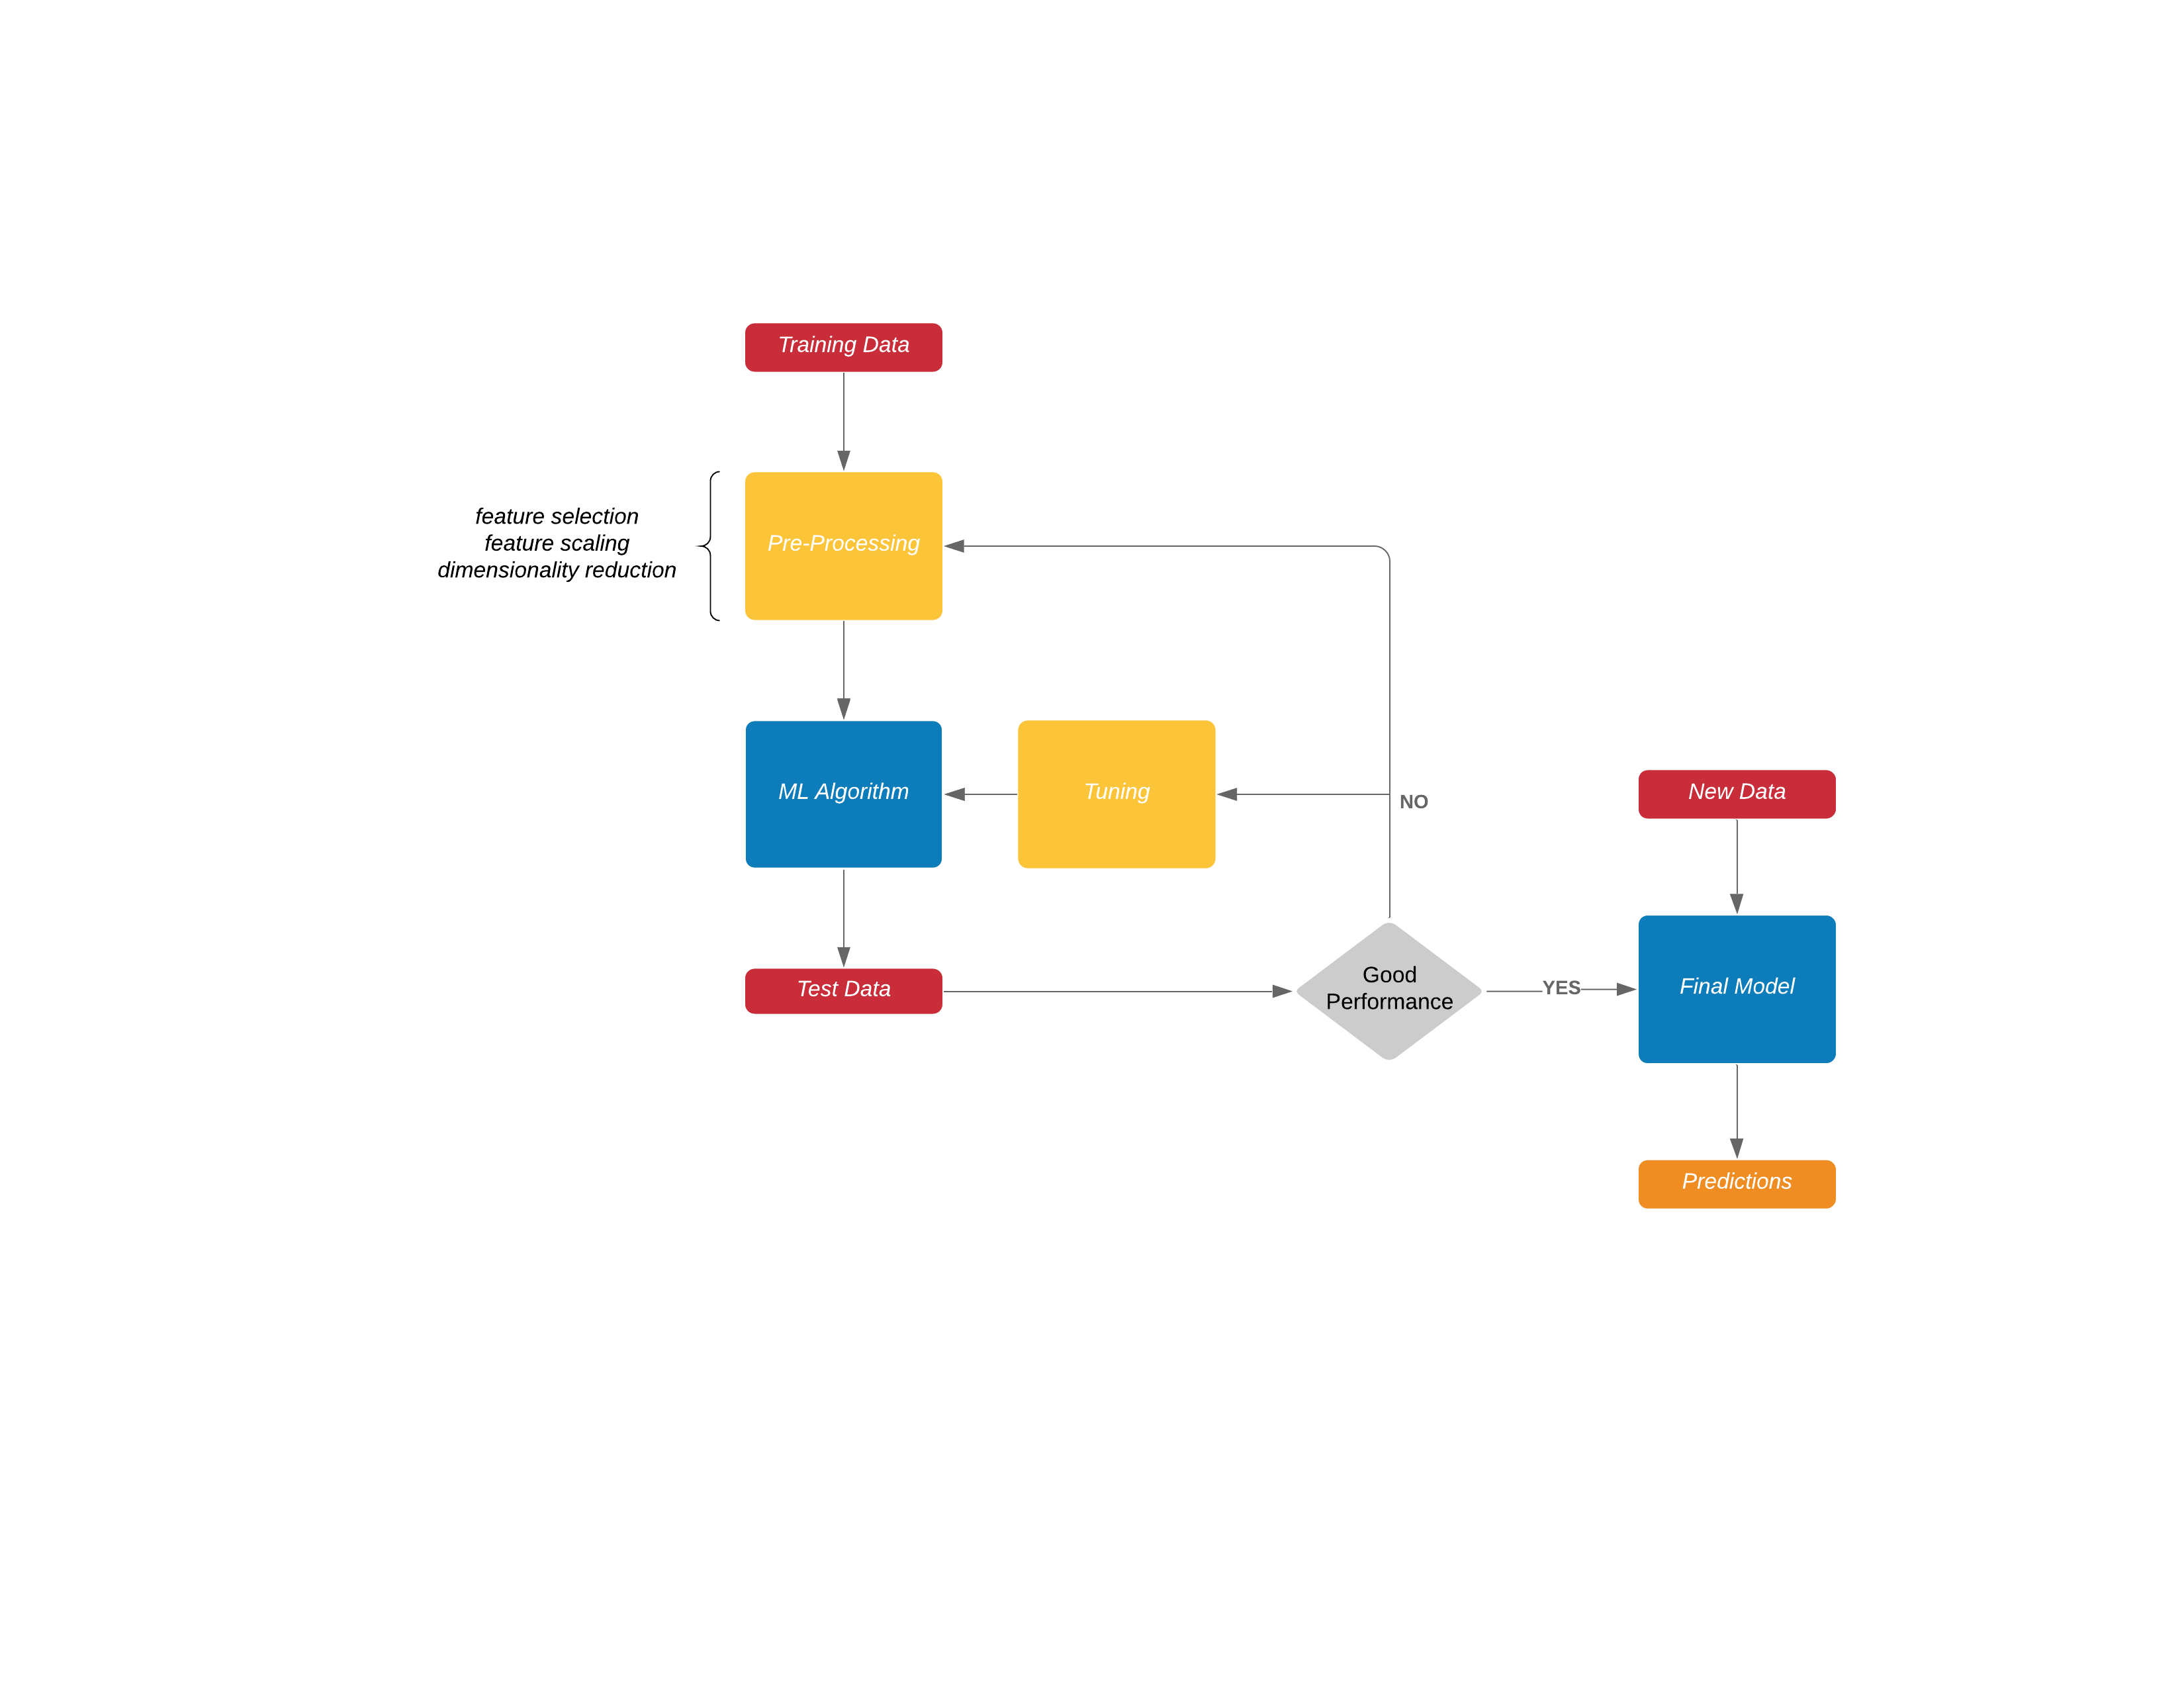
\includegraphics[width=\linewidth]{mlflow.png}
\caption{Supervised machine learning flowchart.}
\label{fig:mlflow}
\end{figure}

\begin{enumerate}
    \item Split the data into training data and testing data.
    \item Process the training data via feature selection, feature scaling, dimensionality reduction, etc. to simplify the model, reduce training time, and improve performance.
    \item Choose a machine learning algorithm and use the training data to build a predictive model.
    \item Evaluate the performance of the predictive model on new, unseen test data.
    \item If the model achieves the desired performance, then new data can be used as input to the final model to produce predictions. Otherwise, go back to the preprocessing step or tune the hyperparameters of the machine learning algorithm and build a new model.
    \item Repeat until the desired performance is reached.
\end{enumerate}

Many different machine learning algorithms can be substituted in the third step, which is why supervised machine learning is known as an ill-posed problem \cite{mitfundamentals}. No one machine learning algorithm is universally the best in every application; every algorithm has its own set of assumptions (inductive bias) that make it better or worse in certain situations.

Previous models built to predict wins using team statistics have used the linear regression algorithm. In addition to linear regression, I use other machine learning algorithms, specifically regression trees and $k$-nearest neighbors, to learn non-linear relationships in the data and attempt to improve model performance. Next, I briefly describe how each of these techniques works.

\subsection{Linear Regression}

Linear regression assigns a set of weights, one for each descriptive feature, to combine them into a prediction for the target variable. The first step in linear regression is to plot each instance in the training data in an $m$-dimensional feature space, where $m$ is the total number of features and each feature defines an axis. Then, an optimal set of weights is calculated to fit a hyperplane closest to all the data points \cite{regtechniques}. The best-fit hyperplane is the one that minimizes the average squared distance of each data point to the hyperplane as shown in Figure \ref{fig:linreg}. The best-fit hyperplane can then be used to make predictions for a new instance by finding the point on the hyperplane closest to the instance in the feature space.

\begin{figure}[hbt]
\centering
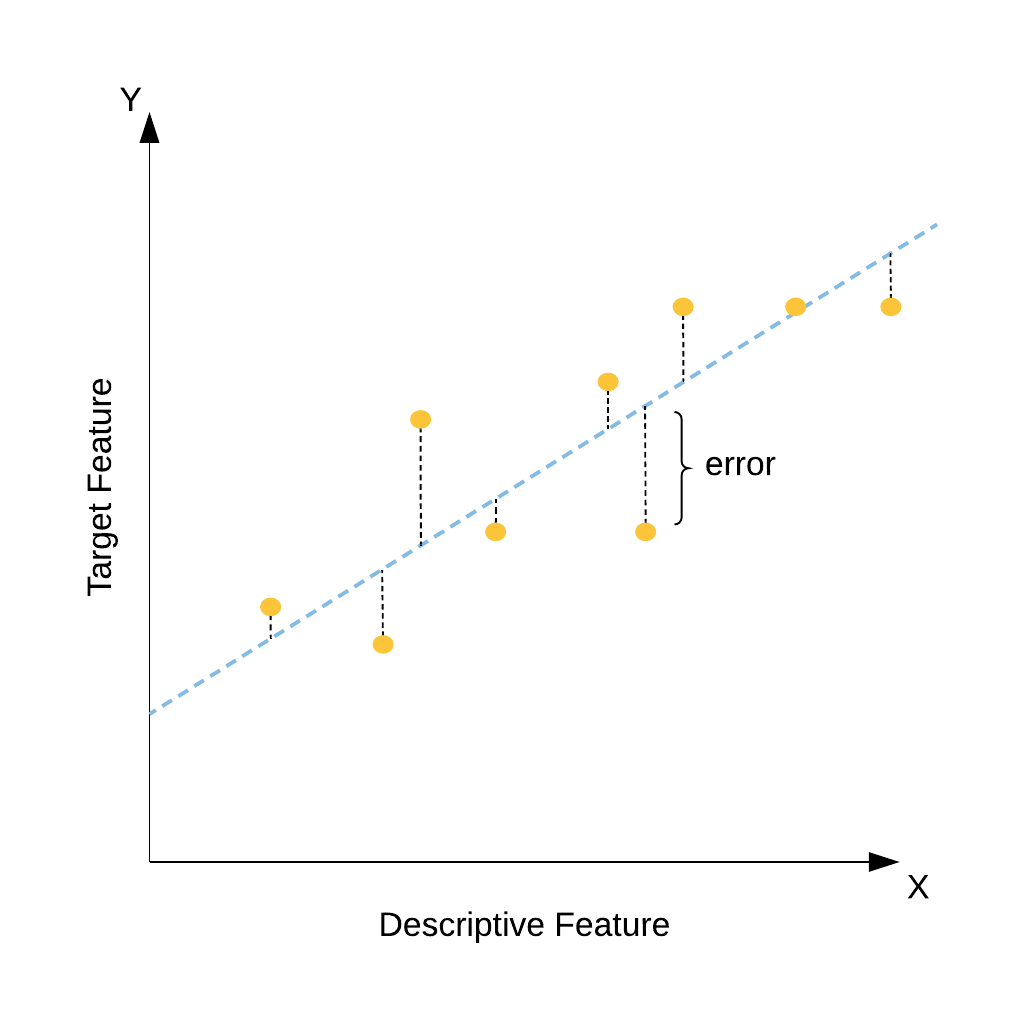
\includegraphics[width=0.5\linewidth]{linreg.png}
\caption{The best-fit hyperplane minimizes $\frac{1}{n}\sum\text{error}^2$.}
\label{fig:linreg}
\end{figure}

\subsection{k-Nearest Neighbors (k-NN)}

The idea behind $k$-NN is that instances with similar descriptive feature values should have similar target feature values. Just like linear regression, $k$-NN begins by plotting the training instances in the feature space. However, in $k$-NN, the feature space is defined by only the descriptive features. Then, to produce a prediction for a new instance, as the name suggests, the algorithm finds the $k$ closest training instances (which should be most similar to the new instance) and generates a distance-weighted average of the target values for those $k$ instances \cite{mitfundamentals}. An example is illustrated in Figure \ref{fig:knn}. The "X" indicates the new query instance we are making a prediction for and the blue dots represent the training instances. In this example, $k=3$, so the prediction would be a distance-weighted average of the target values for the three circled blue dots where the weight for the $i$th dot would be $\frac{1}{d(q,d_i)^2}$ \cite{mitfundamentals}. Here, $d(q,d_i)$ designates the distance between the query instance and the $i$th dot.

\begin{figure}[hbt]
\centering
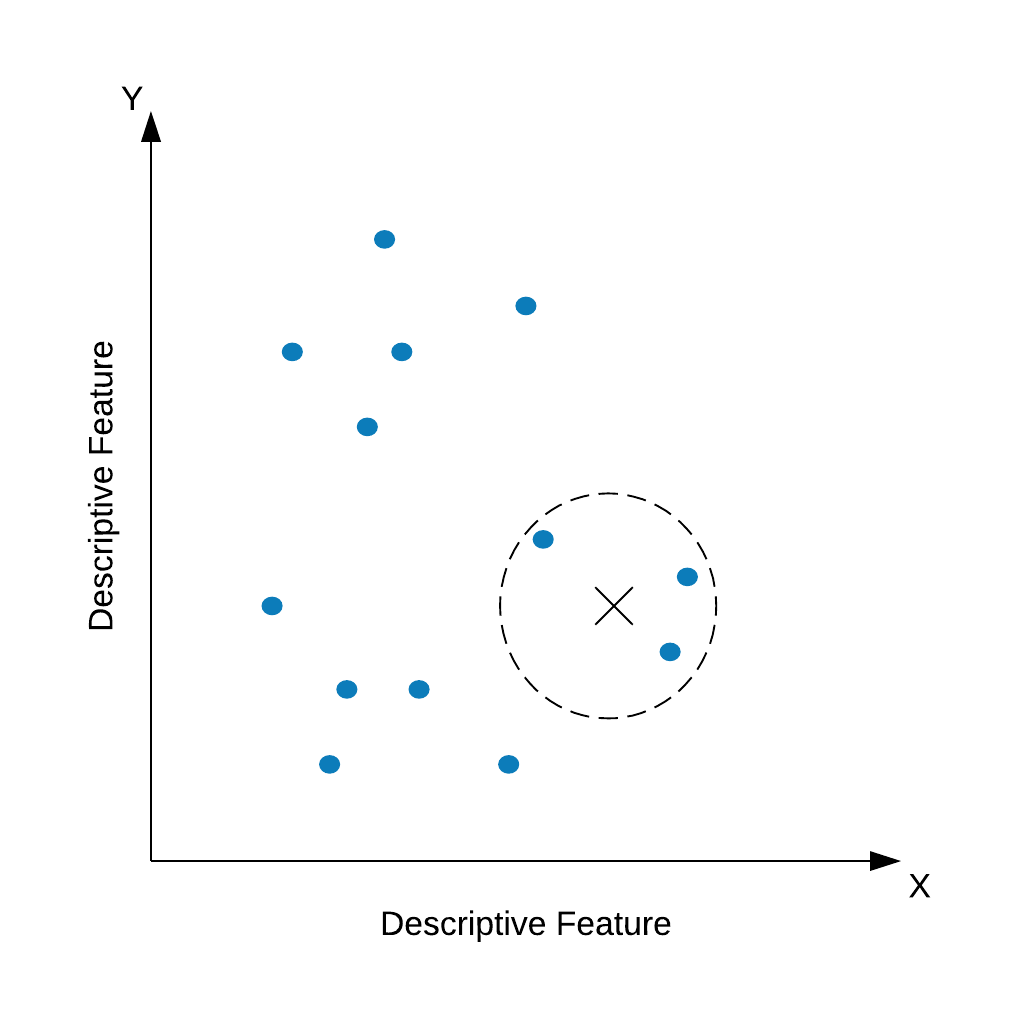
\includegraphics[width=0.5\linewidth]{kNN.png}
\caption{k-Nearest Neighbors for k=3.}
\label{fig:knn}
\end{figure}

\subsection{Regression Trees}

Knowing how a regression tree generates predictions makes it easier to understand how to build one. Regression trees produce estimates by using a series of binary decisions that repeatedly split the data into narrower groups of target values until the variability in the set of possible values is low enough for the model to make a confident prediction \cite{trees}. At each internal node, a descriptive feature value is tested (i.e. lower or higher than some threshold) and the algorithm traverses the three left or right based on the result of each test until a leaf node is reached. Each leaf node represents a partition of the original data which contains instances with similar descriptive feature values. The final prediction produced is an average of the target feature values for the instances in that leaf node \cite{trees}.
For example, Figure \ref{fig:regtrees} shows a regression tree built to predict the temperature given the latitude and elevation of a particular location. To make a prediction for the temperature at a new location, the algorithm starts at the root node and first checks the latitude (how far the location is from the equator). Then it tests the elevation (how far above sea level the location is). Based on these two tests, the algorithm reaches a leaf node and returns the average temperature for the instances in that leaf node. 

Regression trees are constructed in a recursive, depth-first manner. At each internal node, a feature and threshold are chosen to maximize the reduction in entropy (minimize variability/uncertainty) in the target feature values for the resulting partitions \cite{mitfundamentals}. This process is repeated until some stopping condition holds and a leaf node is created. Examples of such stopping conditions include:

\begin{itemize} 
    \item Instances in a partition have the same target value or have sufficiently low variability.
    \item The tree has reached a predetermined maximum depth.
    \item All descriptive features and thresholds have been tested along a branch.
\end{itemize}

\begin{figure}[hbt]
\centering
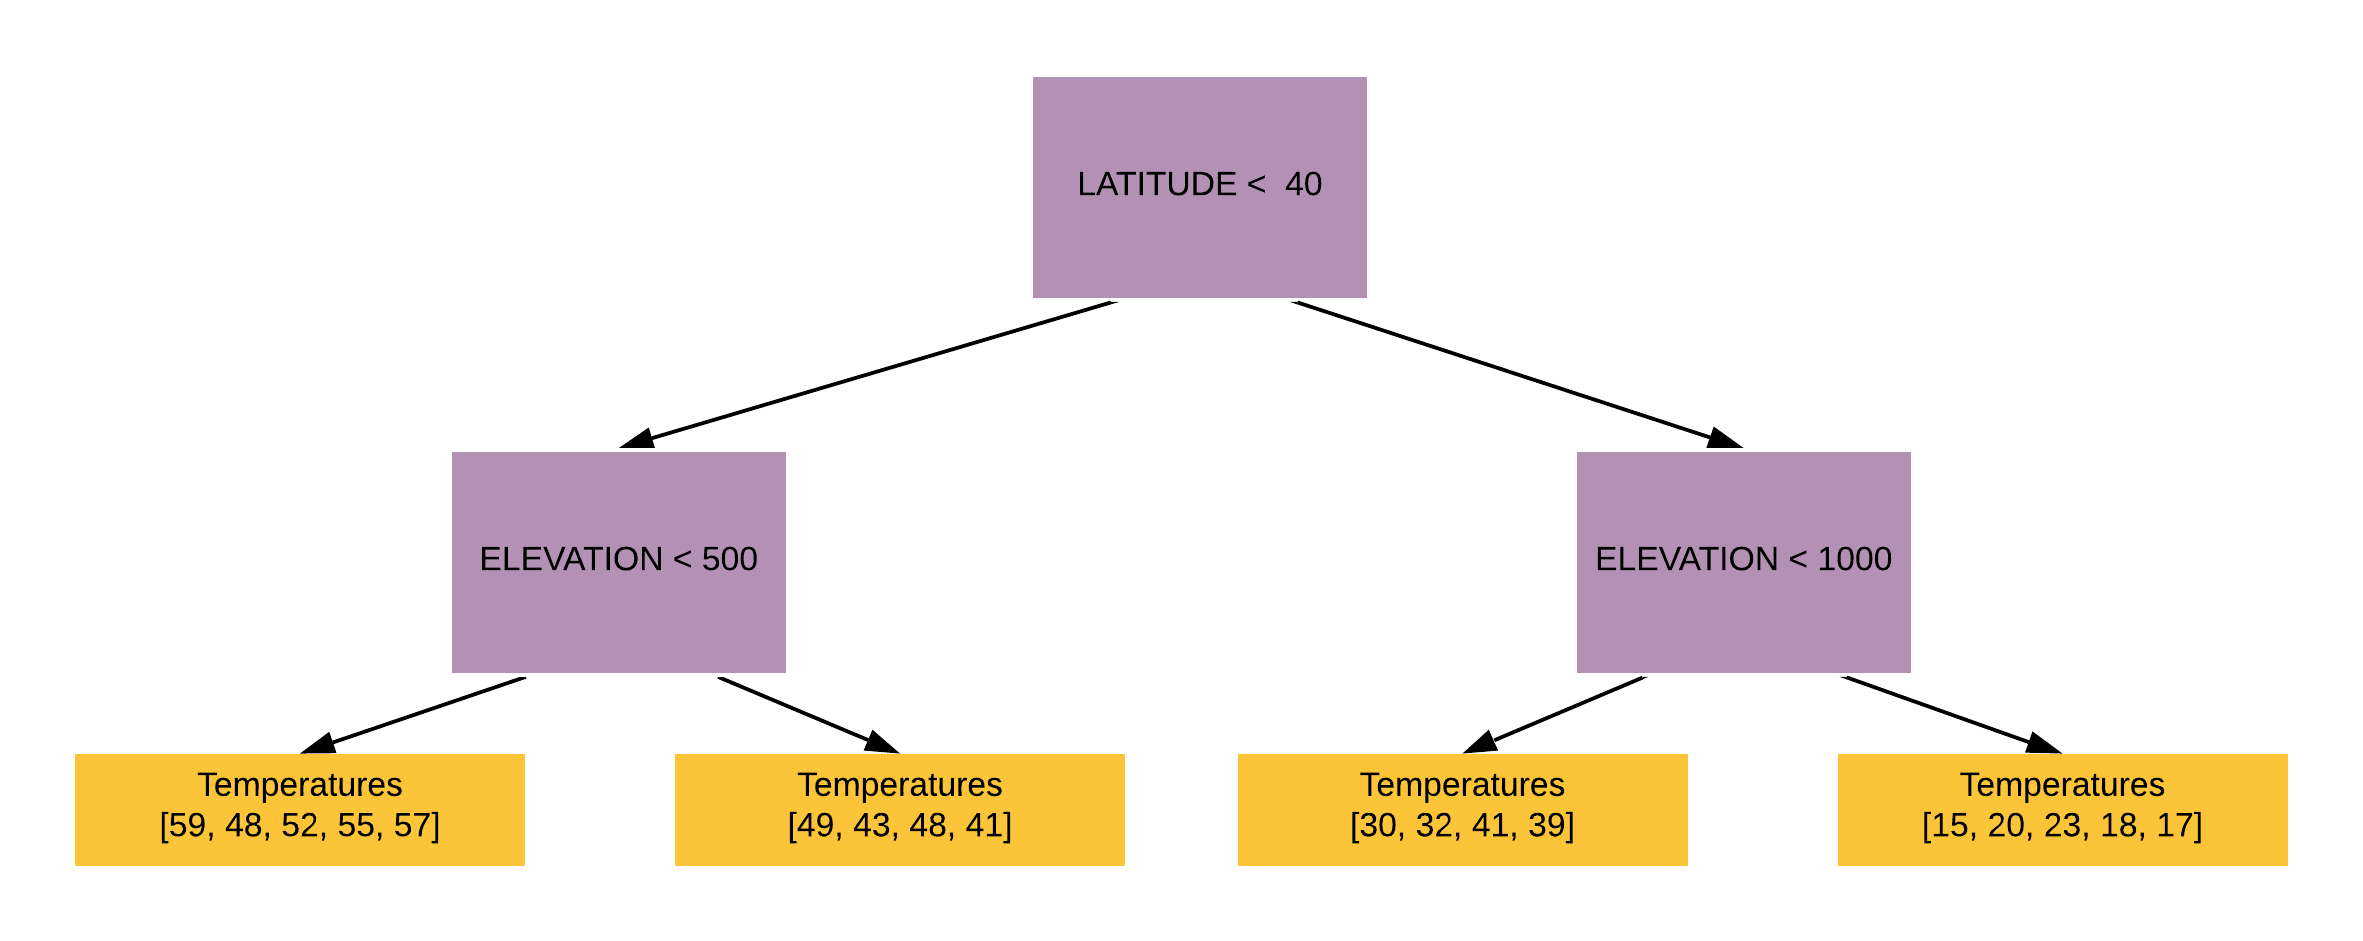
\includegraphics[width=\linewidth]{regtrees.png}
\caption{Regression tree for predicting temperature based on a location's latitude and elevation.}
\label{fig:regtrees}
\end{figure}

\subsection{Choosing the Best Model}

The performance of machine learning models can vary greatly depending on the preprocessing techniques and hyperparameters used to build them. The goal of model selection is to evaluate and compare the performance of different models and choose the one that performs best. As mentioned earlier in the supervised machine learning discussion, a predictive model is built using training data but evaluated using test data. A model that makes accurate predictions on test data that it has not seen before is said to generalize well \cite{mitfundamentals}. The best models generalize and perform well on test data and so should also perform well on any other new data.

Predictive models that do not generalize well face problems such as underfitting and overfitting. Underfitting occurs when the model is too simple; it does not capture the full relationship between the descriptive features and target feature. Overfitting occurs when the model "memorizes" the training data instead of learning the relationships between variables; the model fits too closely to the training data and is affected by noise and patterns specific to the training data \cite{mitfundamentals}. The difference between underfitting and overfitting is illustrated in Figure \ref{fig:fit}.

\begin{figure}[hbt]
\centering
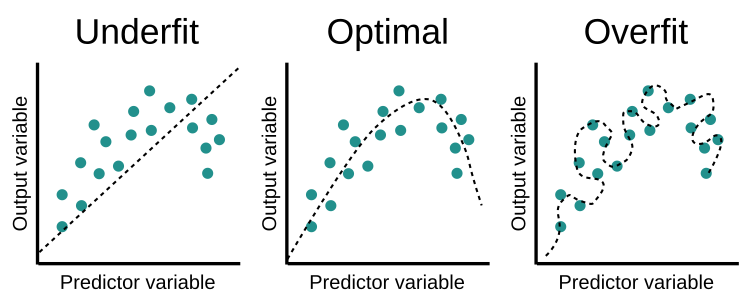
\includegraphics[width=0.75\linewidth]{fit.png}
\caption{A good model strikes a balance between simplicity and complexity.\\
Source: \cite{fit}}
\label{fig:fit}
\end{figure}

One way to monitor for underfitting and overfitting when training models is to plot training error and testing error for models of increasing complexity. Models generally improve (training and testing error decrease) with increasing complexity until a point at which the model begins overfitting (testing error increases while training error continues to decrease). The best model complexity occurs at the inflection point when testing error begins to increase. This pattern is shown in Figure \ref{fig:traintest}. 

\begin{figure}[hbt]
\centering
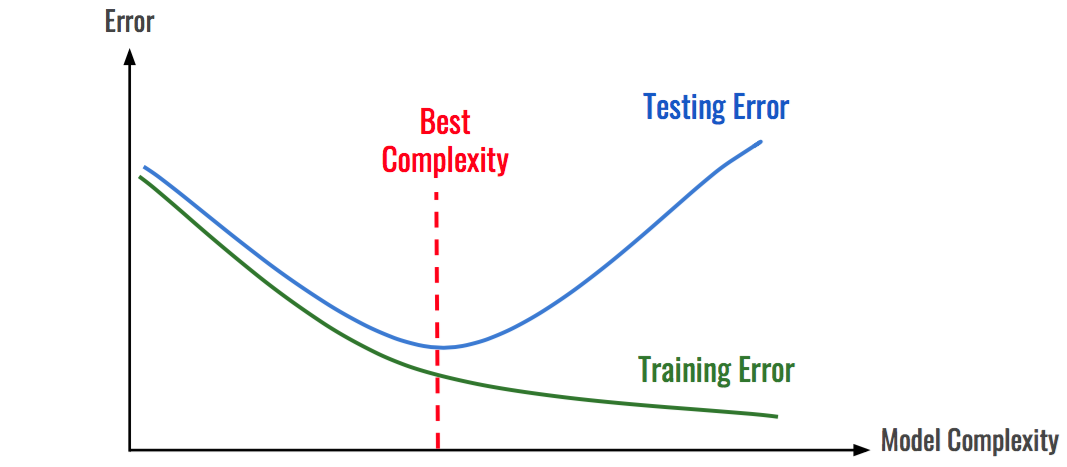
\includegraphics[width=0.75\linewidth]{traintest.png}
\caption{Monitoring for goodness of fit by plotting testing and training error.\\
Source: \cite{traintest}}
\label{fig:traintest}
\end{figure}

Model building is a balancing act and comes with many considerations. In the Implementation selection, I go into more detail on how I gather my data and split it into train, test, and validation sets for separately building and then evaluating the models. I also describe how I use each of the three machine learning algorithms in combination with hyperparameter tuning and a variety of preprocessing techniques to improve model performance.

\section{Implementation}

At a high level, this project can be broken down into three stages: data preparation, model building, and model evaluation/selection.

\begin{figure}[hbt]
\centering
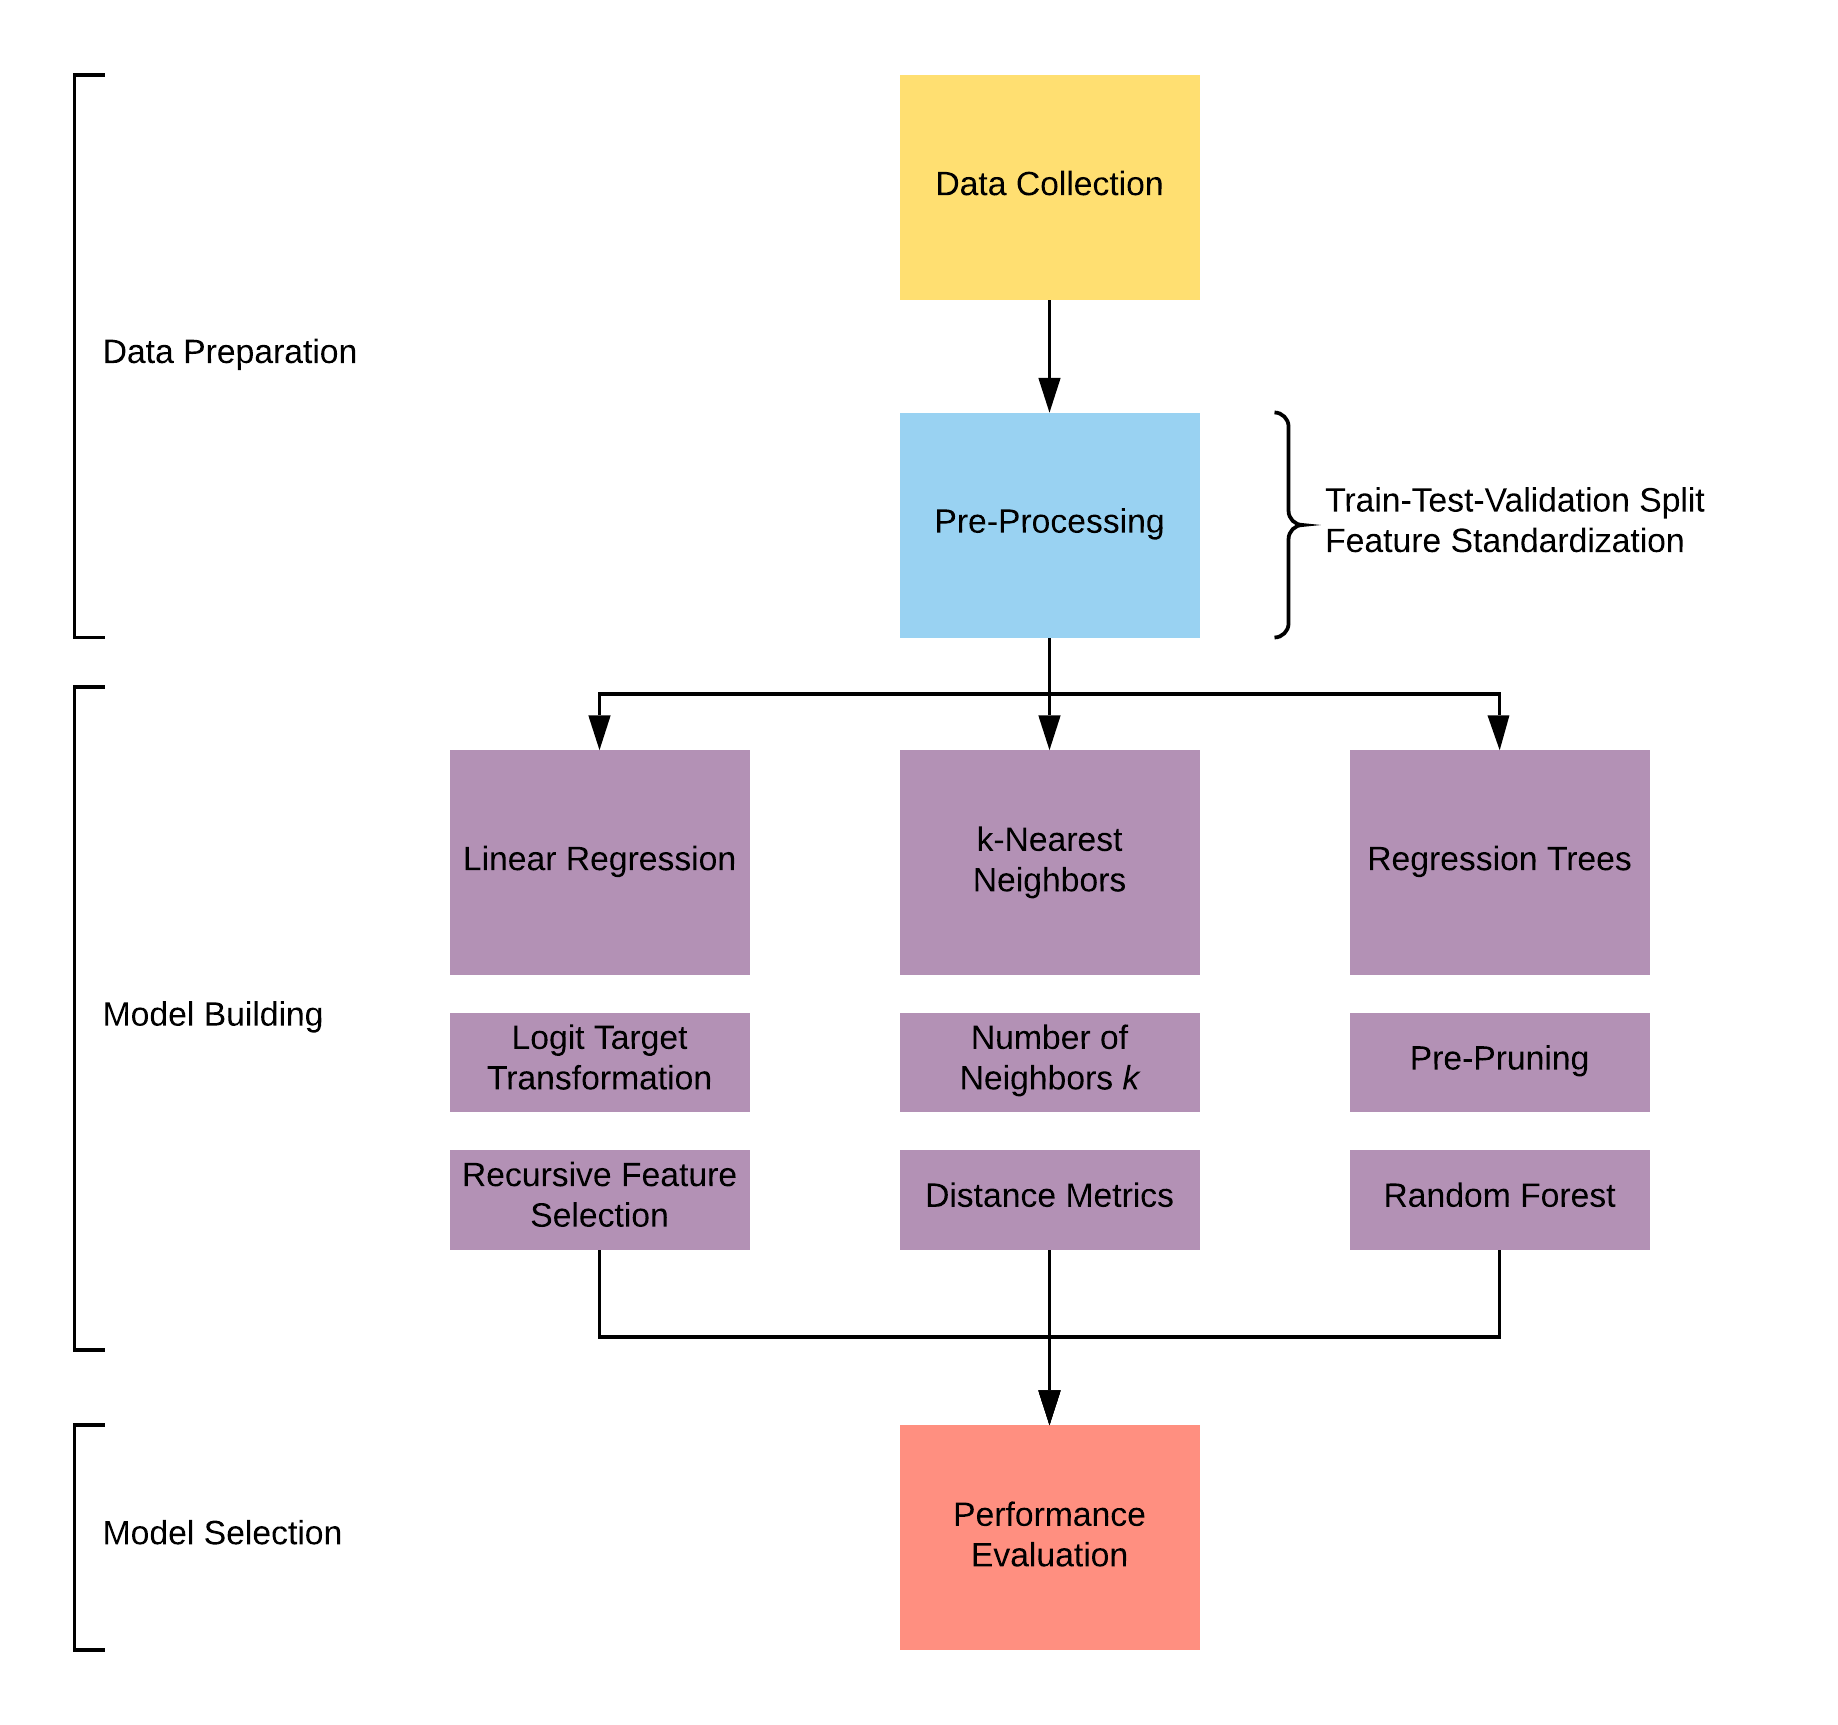
\includegraphics[width=0.75\linewidth]{implementation.png}
\caption{Implementation overview.}
\label{fig:implementation}
\end{figure}

An overview of these stages and the steps that comprise each one is shown in Figure \ref{fig:implementation}. This section discusses the specifics of the data preparation and model building stages.

\subsection{Data Preparation}

The data used in this project includes 19 team statistics and winning percentage, a total of 20 data points, for every team in the league from 1980-1981 to 2018-2019. The full list of team statistics and descriptions is shown in Table~\ref{table:statistics}.

\begin{table}[hbt]
  \centering
  \begin{tabular}{|l|l|}
    \hline
    \textbf{Statistic} & \textbf{Description}\\
    \hline
    FGA & Shots attempted per game\\
    \hline
    3PA & 3-pointers attempted per game\\
    \hline
    AST & Assists per game\\
    \hline
    OPP\_FGA & Opponent shots attempted per game\\
    \hline
    OPP\_3PA & Opponent 3-pointers attempted per game\\
    \hline
    OPP\_AST & Opponent assists per game\\
    \hline
    WINS\_PYTH & Expected wins based on points scored and allowed \\
    \hline
    LOSSES\_PYTH & Expected losses based on points scored and allowed\\
    \hline
    MOV & Margin of victory\\
    \hline
    NRTG & Estimate of point differential per 100 possessions\\
    \hline
    TS\_PCT & Shooting efficiency\\
    \hline
    EFG\_PCT & Effective field goal percentage\\
    \hline
    TOV\_PCT & Estimate of turnovers committed per 100 plays\\
    \hline
    ORB\_PCT & Estimate of percentage of available offensive rebounds grabbed\\
    \hline
    FT\_RATE & Free throws attempted per field goal attempted\\
    \hline
    OPP\_EFG\_PCT & Opponent effective field goal percentage\\
    \hline
    OPP\_TOV\_PCT & Turnovers committed by opponent per 100 plays\\
    \hline
    DRB\_PCT & Estimate of percentage of available defensive rebounds grabbed\\
    \hline
    OPP\_FT\_RATE & Opponent free throws attempted per field goal attempted\\
    \hline
  \end{tabular}
  \caption{Statistical descriptions.}
  \label{table:statistics}
\end{table}

All the data was scraped from Basketball Reference \cite{bballref} using BeautifulSoup \cite{soup} to parse the HTML and Selenium \cite{selenium} to navigate between webpages for different seasons. I withheld the data for the 2018-2019 season for use as validation data and the remaining data I randomly divided into train and test sets using an 80-20 split. After the split, the training data contains data for 835 teams and the training data contains data for 209 teams.

For preprocessing, I standardized the descriptive feature values in the training set to have a mean of zero and unit variance. Then I applied the same transformation to the testing data. I performed the train-test split and feature standardization using Scikit-learn \cite{scikit-learn}.

\subsection{Linear Regression}

Before building an optimized linear regression model, I fit a baseline model using all 19 team statistics. The model ended up producing negative winning percentage predictions and predictions over one. To correct this, I scaled the target values in the data using the logit function, which transforms values in the range $[0, 1]$ to $(-\infty, \infty)$. I then used this transformed data to train the model to produce logit winning percentage predictions. Then, to convert those predictions back to normal winning percentages in $[0, 1]$, I used the logistic function \cite{wikilogit,stackoverflow}.

To try and improve upon the performance of the baseline model, I used recursive feature selection to trim the number of team statistics used to build the model.
Recursive feature selection works by first training the model on the full set of features. Then it recursively considers smaller and smaller sets of features, pruning the least important feature at each step. This process is repeated until the desired number of features is reached. Feature selection has the benefits of reducing dimensionality, simplifying the model, and limiting overfitting. To settle on the optimal number of features, I built 19 models, varying the number of features from 1 to all 19. For each model, I plotted the training and testing error shown in Figure \ref{fig:featureselect}. This plot shows that, interestingly, performance does not improve beyond two features and even the improvement going from one to two features is very slight.

\begin{figure}[hbt]
\centering
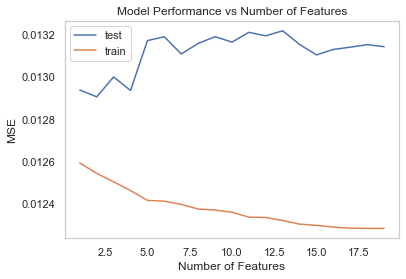
\includegraphics[width=0.75\linewidth]{featureselect.png}
\caption{Linear regression model performance using different numbers of features.}
\label{fig:featureselect}
\end{figure}

The best model, which uses two features, has the best-fit hyperplane equation below and can be visualized in Figure \ref{fig:bestlinear}. $$\text{logit}\left(W/L\%\right) = 1.059 * MOV - 0.6109 * NRTG + 0.01467$$

\begin{figure}[hbt]
\centering
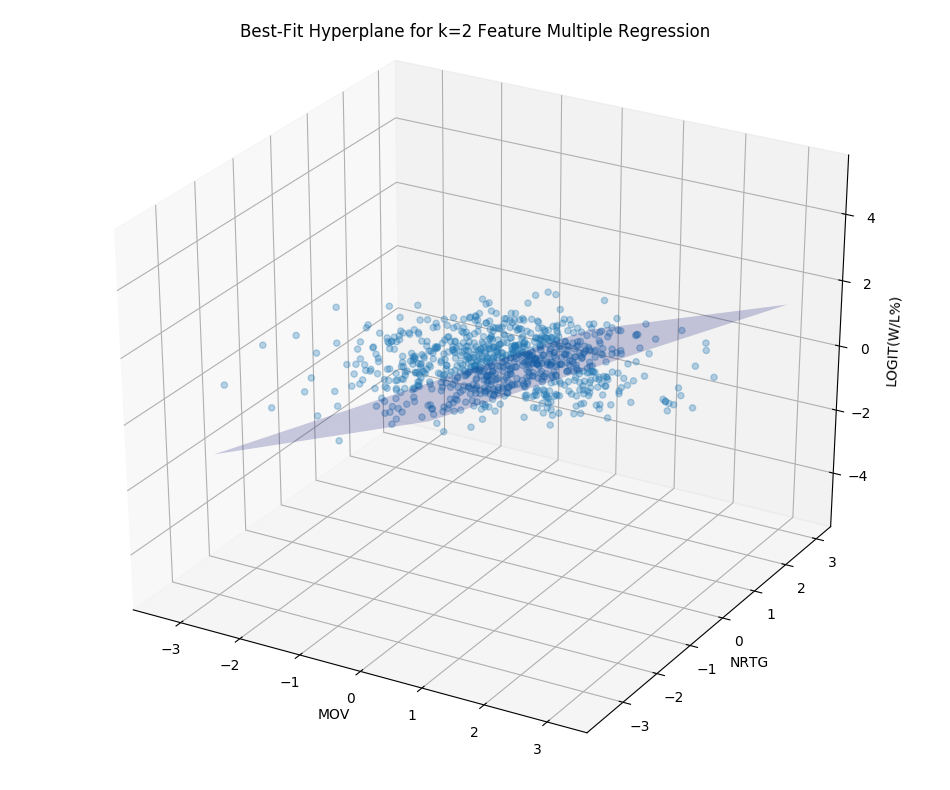
\includegraphics[width=0.75\linewidth]{bestlinear.png}
\caption{Visualization of linear regression model using 2 features.}
\label{fig:bestlinear}
\end{figure}

\newpage 

\subsection{k-Nearest Neighbors}

I used two parameters to adjust the performance of a $k$-NN model: number of neighbors $k$ and distance metric. I first built a standard model using the default parameters ($5$ neighbors and Euclidean distance). This model, as expected, resulted in significant overfitting, so I used hyperparameter tuning to find the best-performing distance metric and value of $k$. For distance metric, I compared Euclidean and Manhattan. The Euclidean metric measures the straight-line distance between two points $a$ and $b$ in an $m$-dimensional space according to $\sqrt{\sum_{i=1}^{m}(a[i]-b[i])^2}$ and the Manhattan metric measures the shortest grid-like distance according to $\sum_{i=1}^{m}abs(a[i]-b[i])$ \cite{mitfundamentals}. Figure \ref{fig:distmetric} compares the testing error of models using Euclidean and Manhattan distance for different values of $k$. This plot shows that using the Manhattan metric decreases error on the test set and improves performance. 

\begin{figure}[hbt]
\centering
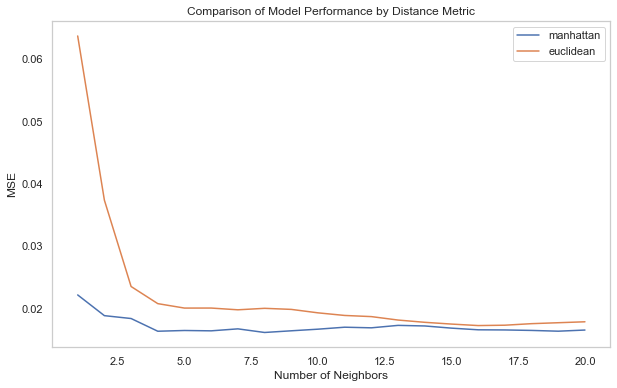
\includegraphics[width=0.75\linewidth]{distmetric.png}
\caption{Comparison of k-NN model performance using Euclidean and Manhattan metrics.}
\label{fig:distmetric}
\end{figure}

To find the optimal value of $k$, I plotted training and testing error of Manhattan models for increasing values of $k$. As shown in Figure \ref{fig:manhattan}, model performance improves until $k$ reaches $5$ and then plateaus. The results of hyperparameter tuning combine to yield a final $k$-NN model that uses Manhattan distance and $k=5$ neighbors.

\begin{figure}[hbt]
\centering
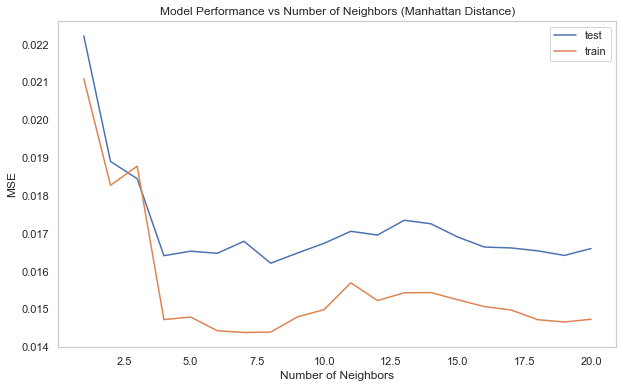
\includegraphics[width=0.75\linewidth]{manhattan.png}
\caption{Manhattan k-NN model performance using different numbers of neighbors.}
\label{fig:manhattan}
\end{figure}

\subsection{Regression Trees/Random Forest}

To build an optimized regression tree, I started again by building a baseline model. With no limit on the maximum depth, the complexity of this model allowed it to achieve perfect performance on the training set. However, high testing error suggested overfitting. To simplify the model, I used an approach known as pre-pruning to limit the maximum tree depth \cite{mitfundamentals}. Figure \ref{fig:treedepth} shows the performance of various regression trees with maximum depths ranging from 1 to 25. As seen in the figure, model performance improves with increasing depth until maximum depth exceeds 3, at which point testing error begins to increase. The optimized regression tree with a maximum depth of 3 is displayed in Figure \ref{fig:bestsingletree}. 

\begin{figure}[hbt]
\centering
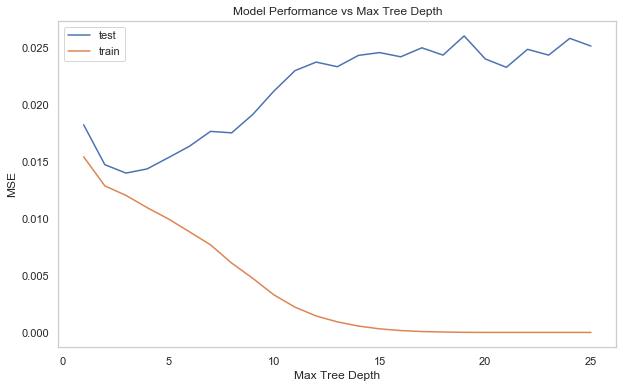
\includegraphics[width=0.75\linewidth]{treedepth.png}
\caption{Regression tree performance using different max depths.}
\label{fig:treedepth}
\end{figure}

\begin{figure}[hbt]
\centering
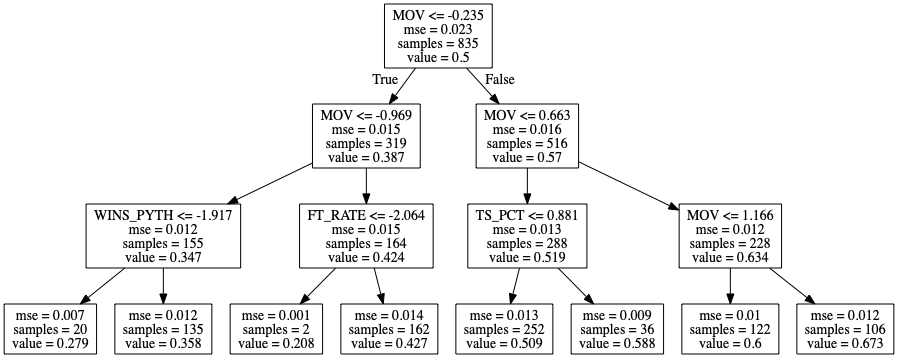
\includegraphics[width=\linewidth]{bestsingletree.png}
\caption{Regression tree with max depth of 3.}
\label{fig:bestsingletree}
\end{figure}

The single regression tree still produced relatively high error on the testing set, so I implemented an extension of regression trees known as random forest. Random forest is an example of a model ensemble approach which means that it uses the predictions of a set of models to produce an aggregate prediction. To ensure that all the models do not produce the same prediction, the random forest algorithm trains each model on different data by sampling with replacement from the training set and using subspace sampling to vary the set of features used \cite{mitfundamentals}. To find the optimal number of trees and maximum depth for each tree, I used hyperparameter tuning in two steps. First, I performed a broad, randomized search that tried values ranging from 10 to 1000 for the number of estimators and depths of 1 to 24 for each individual tree. Then using these results, I performed a more refined search over the parameter space that tried a narrower range of values for number of trees and maximum depth \cite{hyperparam}. The best random forest model that resulted from these searches used 600 trees and each tree had a maximum depth of 3.

\section{Evaluation}

The evaluation section is divided into three parts. First, I describe which performance metrics I used to compare the models and how to interpret them. Then I choose the model with the best performance as the final model and evaluate it on the validation set and use it to make predictions for the current 2019-2020 season. Lastly, I discuss which features appear to be most important in these models.

\subsection{Performance Metrics and Model Evaluation}

To evaluate model performance, I used mean squared error and root mean squared error on the test set. If we define error to be the difference between the predicted winning percentage and the actual winning percentage for an instance,
then mean squared error is the average squared error for the entire training set and root mean squared error is the square root of mean squared error \cite{mitfundamentals}. To summarize, the formulas for mean squared error (mse) and root mean squared error (rmse) are given below.

$$MSE = \frac{1}{n}\sum_{t=1}^{n}error^2$$
$$RMSE = \sqrt{MSE} = \sqrt{\frac{1}{n}\sum_{t=1}^{n}error^2}$$

The benefit of taking the extra step to calculate root mean squared error is that it has the same units as the target variable, making it easier to interpret. Going one step further, multiplying root mean squared error by 82 gives the average error in terms of number of games. 

\begin{table}[hbt]
  \centering
  \begin{tabular}{|cccc|}
    \hline
    & \textbf{Linear} & \textbf{k-NN} & \textbf{Random Forest}\\
    \hline
    \textbf{MSE} & 0.0129 & 0.0165 & 0.0136\\
    \textbf{RMSE} & 0.1137 & 0.1286 & 0.1166\\
    \textbf{No. Games} & 9.3234 & 10.5443 & 9.5612\\
    \hline
  \end{tabular}
  \caption{Performance comparison.}
  \label{table:errors}
\end{table}

The mean squared error, root mean squared error, and equivalent number of games for the best linear, k-NN, and random forest models are given in Table~\ref{table:errors}. The best model, the one that minimizes error, turns out to be the linear model.

Figure \ref{fig:actualvspredicted} gives a closer look at the best linear model's performance. A perfect model makes predictions along the $y=x$ line shown in the plot, which represents all points for which actual winning percentage equals predicted winning percentage. Here we see points spread above and below the line with a few outliers.

\begin{figure}[hbt]
\centering
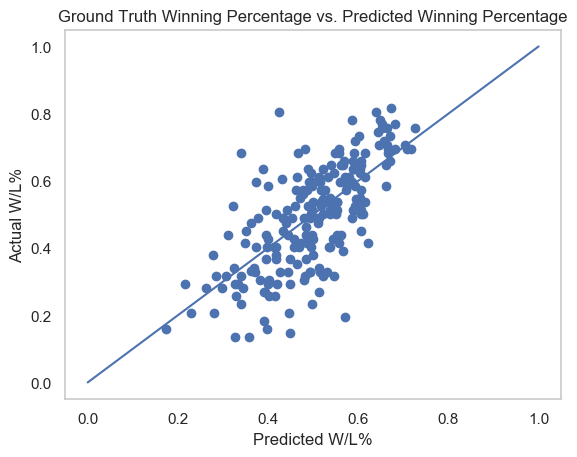
\includegraphics[width=0.75\linewidth]{actualvspredicted.png}
\caption{Regression tree performance using different numbers max depths.}
\label{fig:actualvspredicted}
\end{figure}

Figure \ref{fig:residuals} shows a plot of the residuals (actual winning percentage minus predicted winning percentage) for the test set. The residuals plot suggests that the model produces winning percentages that are too high when the actual winning percentage is low and winning percentages that are too low when the actual winning percentage is high.

\begin{figure}[hbt]
\centering
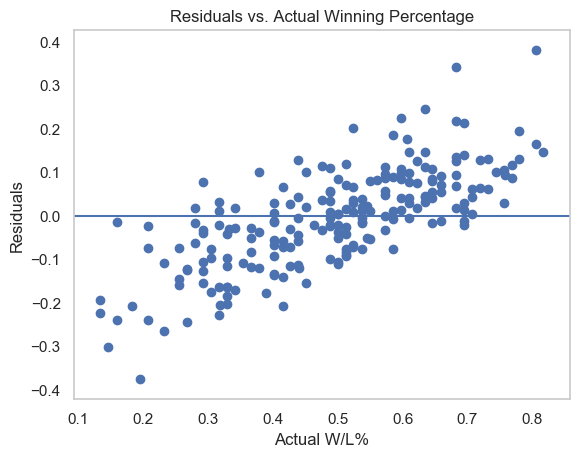
\includegraphics[width=0.75\linewidth]{residuals.png}
\caption{Regression tree performance using different numbers max depths.}
\label{fig:residuals}
\end{figure}

\newpage

\subsection{Validation Performance}

The linear model actually performs better on the validation set than the test set. The model achieves a mean squared error of 0.0108 and a root mean squared error of 0.1042. However, because the validation set contains just 30 instances from the 2018-2019 season, there is likely to be high variability in performance and this should not be taken as a true indication of performance. Instead, this just serves as added confirmation of the linear model's performance.

\subsection{2019-2020 Season Predictions}
\label{section:currentseason}

Table~\ref{table:currentpreds} gives the predictions for the 2019-2020 season next to the projected win totals provided by the sportsbook FanDuel \cite{fanduel} for comparison.

\begin{table}[hbt]
  \centering
  \begin{tabular}{|ccc|}
    \hline
    \textbf{Team} & \textbf{Predicted Wins} & \textbf{FanDuel Projected Wins}\\
    \hline
    \textbf{Milwaukee Bucks} & 59 & 57.5\\
    \textbf{Utah Jazz} & 52 & 54.5\\
    \textbf{Los Angeles Clippers} & 43 & 54.5\\
    \textbf{Philadelphia 76ers} & 47 & 54.5\\
    \textbf{Houston Rockets} & 51 & 53.5\\
    \textbf{Denver Nuggets} & 49 & 53.5\\
    \textbf{Los Angeles Lakers} & 38 & 51.5\\
    \textbf{Boston Celtics} & 51 & 48.5\\
    \textbf{Golden State Warriors} & 55 & 47.5\\
    \textbf{San Antonio Spurs} & 45 & 46.5\\
    \textbf{Portland Trail Blazers} & 50 & 46.5\\
    \textbf{Toronto Raptors} & 54 & 46.5\\
    \textbf{Indiana Pacers} & 48 & 46.5\\
    \textbf{Brooklyn Nets} & 41 & 44.5\\
    \textbf{Miami Heat} & 41 & 43.5\\
    \textbf{Orlando Magic} & 43 & 40.5\\
    \textbf{Dallas Mavericks} & 39 & 40.5\\
    \textbf{New Orleans Pelicans} & 38 & 39.5\\
    \textbf{Sacramento Kings} & 39 & 37.5\\
    \textbf{Detroit Pistons} & 41 & 37.5\\
    \textbf{Minnesota Timberwolves} & 38 & 35.5\\
    \textbf{Atlanta Hawks} & 28 & 33.5\\
    \textbf{Oklahoma City Thunder} & 49 & 32.5\\
    \textbf{Chicago Bulls} & 24 & 32.5\\
    \textbf{Phoenix Suns} & 23 & 28.5\\
    \textbf{Washington Wizards} & 35 & 27.5\\
    \textbf{Memphis Grizzlies} & 36 & 27.5\\
    \textbf{New York Knicks} & 23 & 27.5\\
    \textbf{Cleveland Cavaliers} & 23 & 24.5\\
    \textbf{Charlotte Hornets} & 39 & 23.5\\
    \hline
  \end{tabular}
  \caption{Linear model predictions for 2019-2020 season.}
  \label{table:currentpreds}
\end{table}

It is interesting to note that the biggest discrepancies involve teams like the Los Angeles Clippers, Los Angeles Lakers, and Oklahoma City Thunder. These teams had active offseasons between the 2018-2019 and 2019-2020 seasons and as a result of trades and free agent signings, the Los Angeles Clippers and Los Angeles Lakers acquired significantly more talent while the Oklahoma City Thunder lost talented veterans to rebuild with younger players. Fitting with this explanation, my model, which does not take into account free agency or injuries, predicts significantly fewer wins than FanDuel for the Clippers and Lakers and significantly more wins for the Oklahoma City Thunder. I address more on this issue in the Conclusion section.

\subsection{Feature Importance}

Using recursive feature selection in the linear regression model and pre-pruning in the regression tree model, my project suggests that five team statistics---margin of victory, expected Pythagorean wins, free throw rate, true shooting percentage, and net rating---are most predictive of wins in the following season.

\section{Conclusion}

For this project, I built similarity-based models and regression trees to try and improve upon the previous work done to predict winning percentage based on team statistics using linear regression models. However, my work largely confirms the good performance of linear regression models. At the same time, this project does suggest slightly different statistics to be predictive of wins, namely margin of victory, expected Pythagorean wins, free throw rate, true shooting percentage, and net rating.

True shooting percentage and free throw rate are of particular interest for strategy and roster construction. The importance of true shooting percentage, which measures shooting efficiency by adjusting for the point values of different shots, adds evidence for the power of modern analytics-driven basketball that emphasizes the value and efficiency of the 3-pointer. Moreover, the significance of free throw rate points to the benefits of an aggressive play style that gets to the free throw line often.

\subsection{Limitations and Future Work}

As mentioned in Section~\ref{section:currentseason}, my model does not update with new information like free agency, injuries, and trades that affect the talent that a team can put on the floor. To address this limitation, I could continue using the predictive modeling approach and find a way to parameterize talent and add it to the training data or I could try the simulation-based approach taken by FiveThirtyEight mentioned in Section~\ref{section:prevwork}. These ideas provide possibilities for future study. 

\bstctlcite{bstctl:etal, bstctl:nodash, bstctl:simpurl}
\bibliographystyle{IEEEtran}
\bibliography{references}

\end{document}

